% \documentclass[a4paper,10pt]{article} % or whatever
% \documentclass[letterpaper,10pt]{article} % or whatever
\documentclass{article}

% if you need to pass options to natbib, use, e.g.:
     \PassOptionsToPackage{numbers, compress}{natbib}

\usepackage[preprint]{notes}

\newcommand{\ignore}[1]{}
% to avoid loading the natbib package, add option nonatbib:
\usepackage{dsfont}

% Note: this has been tested using MiKTeX 2.9. If you are getting errors, update your packages.

%%% Packages %%%
%\usepackage{setspace} % Double spaces document. Footnotes,
                      % figures, and tables will still be single spaced, however.
%\doublespacing
%\singlespacing
%\onehalfspacing
% \setstretch{1.5} % set double spacing to 1.5 or anything else.

\usepackage[T1]{fontenc}
\usepackage{amsmath,amssymb,amsfonts,mathrsfs,bm}% Typical maths resource packages
\usepackage{mathtools}
%\let\proof\relax
%\let\endproof\relax
\usepackage{amsthm}
\usepackage{nicefrac}
%\usepackage{cite}
%\let\labelindent\relax
\usepackage[shortlabels]{enumitem}
\usepackage{graphicx}
\usepackage{epstopdf}
\usepackage{url}
\usepackage{colortbl}
\usepackage{booktabs}
\usepackage{multirow}
\usepackage[table,dvipsnames]{xcolor}
\usepackage[normalem]{ulem}
\usepackage{xparse}

%\usepackage{pstricks}
%\usepackage{psfrag}
%\usepackage{syntonly}
%\syntaxonly
%\usepackage[style=base]{caption}
%\captionsetup{
    %format = plain,
    %font = footnotesize,
    %labelfont = sc
%}


\usepackage{array}
\newcolumntype{L}[1]{>{\raggedright\let\newline\\\arraybackslash\hspace{0pt}}m{#1}}
\newcolumntype{C}[1]{>{\centering\let\newline\\\arraybackslash\hspace{0pt}}m{#1}}
\newcolumntype{R}[1]{>{\raggedleft\let\newline\\\arraybackslash\hspace{0pt}}m{#1}}

\makeatletter
\let\MYcaption\@makecaption
\makeatother
\usepackage[font=footnotesize]{subcaption}
\makeatletter
\let\@makecaption\MYcaption
\makeatother


% achieves the functionality of \tag for subequations environment
\makeatletter
\newenvironment{varsubequations}[1]
 {%
  \addtocounter{equation}{-1}%
  \begin{subequations}
  \renewcommand{\theparentequation}{#1}%
  \def\@currentlabel{#1}%
 }
 {%
  \end{subequations}\ignorespacesafterend
 }
\makeatother


\usepackage{glossaries}

\makeatletter
% copy old \gls and \glspl
\let\oldgls\gls
\let\oldglspl\glspl

% define a non space skipping version of \@ifnextchar
\newcommand\fussy@ifnextchar[3]{%
  \let\reserved@d=#1%
  \def\reserved@a{#2}%
  \def\reserved@b{#3}%
  \futurelet\@let@token\fussy@ifnch}
\def\fussy@ifnch{%
  \ifx\@let@token\reserved@d
    \let\reserved@c\reserved@a 
  \else
    \let\reserved@c\reserved@b
  \fi
 \reserved@c}

\renewcommand{\gls}[1]{%
  \oldgls{#1}\fussy@ifnextchar.{\@checkperiod}{\@}}
\renewcommand{\glspl}[1]{%
  \oldglspl{#1}\fussy@ifnextchar.{\@checkperiod}{\@}}

\newcommand{\@checkperiod}[1]{%
  \ifnum\sfcode`\.=\spacefactor\else#1\fi
}
\makeatother

%%%%%%%%%%%%% new add %%%%%%%%%%%%% 
\newcommand{\tb}[1]{\textbf{#1}}


\newacronym{wrt}{w.r.t.}{with respect to}
\newacronym{RHS}{R.H.S.}{right-hand side}
\newacronym{LHS}{L.H.S.}{left-hand side}
\newacronym{iid}{i.i.d.}{independent and identically distributed}
%\newacronym{MIMO}{MIMO}{mulitple-input multiple-output}
%\newacronym{AOA}{AOA}{angle-of-arrival}
%\newacronym{AOD}{AOD}{angle-of-departure}
%\newacronym{LOS}{LOS}{line-of-sight}
%\newacronym{NLOS}{NLOS}{non-line-of-sight}
%\newacronym{TOA}{TOA}{time-of-arrival}
%\newacronym{TDOA}{TDOA}{time-difference-of-arrival}
%\newacronym{RSS}{RSS}{received signal strength}
%\newacronym{GNSS}{GNSS}{Global Navigation Satellite System}
%\newacronym{GSP}{GSP}{graph signal processing}
%\newacronym{ML}{ML}{machine learning}


%put the float package before hyperref and algorithm package after hyperref for hyperref to work correctly with algorithm
\usepackage{float}

\ifx\notloadhyperref\undefined
	\ifx\loadbibentry\undefined
		\usepackage[hidelinks,hypertexnames=false]{hyperref} 
	\else
		\usepackage{bibentry}
		\makeatletter\let\saved@bibitem\@bibitem\makeatother
		\usepackage[hidelinks,hypertexnames=false]{hyperref}
		\makeatletter\let\@bibitem\saved@bibitem\makeatother
	\fi
\else
	\ifx\loadbibentry\undefined
		\relax
	\else
		\usepackage{bibentry}
	\fi
\fi

\usepackage[capitalize]{cleveref}
\crefname{equation}{}{}
\Crefname{equation}{}{}
\crefname{claim}{claim}{claims}
\crefname{step}{step}{steps}
\crefname{line}{line}{lines}
\crefname{condition}{condition}{conditions}
\crefname{dmath}{}{}
\crefname{dseries}{}{}
\crefname{dgroup}{}{}

\crefname{Problem}{Problem}{Problems}
\crefformat{Problem}{Problem~(#2#1#3)}
\crefrangeformat{Problem}{Problems~(#3#1#4) to~(#5#2#6)}

\crefname{Theorem}{Theorem}{Theorems}
\crefname{Corollary}{Corollary}{Corollaries}
\crefname{Proposition}{Proposition}{Propositions}
\crefname{Lemma}{Lemma}{Lemmas}
\crefname{Definition}{Definition}{Definitions}
\crefname{Example}{Example}{Examples}
\crefname{Assumption}{Assumption}{Assumptions}
\crefname{Remark}{Remark}{Remarks}
\crefname{Rem}{Remark}{Remarks}
\crefname{remarks}{Remarks}{Remarks}
\crefname{Appendix}{Appendix}{Appendices}
\crefname{Supplement}{Supplement}{Supplements}
\crefname{Exercise}{Exercise}{Exercises}
\crefname{Theorem_A}{Theorem}{Theorems}
\crefname{Corollary_A}{Corollary}{Corollaries}
\crefname{Proposition_A}{Proposition}{Propositions}
\crefname{Lemma_A}{Lemma}{Lemmas}
\crefname{Definition_A}{Definition}{Definitions}
\crefname{rema}{Remark}{Remarks}
\crefname{exma}{Example}{Examples}
\crefname{assuma}{Assumption}{Assumptions}

\usepackage{crossreftools}
\ifx\notloadhyperref\undefined
	\pdfstringdefDisableCommands{%
			\let\Cref\crtCref
			\let\cref\crtcref
	}
\else
	\relax
\fi

\usepackage{algorithm,algorithmic}
\renewcommand{\algorithmicrequire}{\textbf{Input:}}
\renewcommand{\algorithmicensure}{\textbf{Output:}}

%may cause conflict with some packages like tikz, include manually if desired
%load after hyperref
\ifx\loadbreqn\undefined
	\relax
\else
	\usepackage{breqn} 
\fi



%%%%%%%%%%%%%%%%%%%%%%%%%%%%%%%%%%%%%%%%%%%%%%%%


\interdisplaylinepenalty=2500   % To restore IEEEtran ability to automatically break
                                % within multiline equations, when using amsmath.

%%%%%%%%%%%%%%%%%%%%%%%%%%%%%%%%%%%%%%%%

%Theorem declarations

\ifx\renewtheorem\undefined
% for use in main body
\ifx\useTheoremCounter\undefined
\newtheorem{Theorem}{Theorem}
\newtheorem{Corollary}{Corollary}
\newtheorem{Proposition}{Proposition}
\newtheorem{Lemma}{Lemma}
\else
\newtheorem{Theorem}{Theorem}
\newtheorem{Corollary}[theorem]{Corollary}
\newtheorem{Proposition}[theorem]{Proposition}
\fi

\newtheorem{Definition}{Definition}
\newtheorem{Example}{Example}
\newtheorem{Remark}{Remark}
\newtheorem{Assumption}{Assumption}
\newtheorem{Exercise}{Exercise}

% for use in the appendix
\newtheorem{Theorem_A}{Theorem}[section]
\newtheorem{Corollary_A}{Corollary}[section]
\newtheorem{Proposition_A}{Proposition}[section]
\newtheorem{Lemma_A}{Lemma}[section]
\newtheorem{Definition_A}{Definition}[section]
\fi

\usepackage{amsmath}
\numberwithin{equation}{section} % or whatever you prefer
% \swapnumbers % I prefer this
% \theoremstyle{plain}
\newtheorem{thma}[equation]{Theorem}
\newtheorem{propa}[equation]{Proposition}
\newtheorem{lema}[equation]{Lemma}
\newtheorem{defa}[equation]{Definition}
\newtheorem{cora}[equation]{Corollary}
\newtheorem{Lemma_AA}{Lemma}[section]
\newtheorem{rema}[equation]{Remark}
\newtheorem{exma}[equation]{Example}
\newtheorem{assuma}[equation]{Assumption}
\newcommand{\ml}[1]{\begin{multlined}#1\end{multlined}}
\newcommand{\nn}{\nonumber\\ }


% Remarks
\theoremstyle{remark}
\newtheorem{Rem}{Remark}
\theoremstyle{plain}

\newenvironment{remarks}{
	\begin{list}{\textit{Remark} \arabic{Rem}:~}{
    \setcounter{enumi}{\value{Rem}}
    \usecounter{Rem}
    \setcounter{Rem}{\value{enumi}}
    \setlength\labelwidth{0in}
    \setlength\labelsep{0in}
    \setlength\leftmargin{0in}
    \setlength\listparindent{0in}
    \setlength\itemindent{15pt}
		}
}{
	\end{list}
}


% Special Headings
%\newtheorem*{Prop1}{Proposition 1} %needs amsthm

%\newtheoremstyle{nonum}{}{}{\itshape}{}{\bfseries}{.}{ }{#1 (\mdseries #3)}
%\theoremstyle{nonum}
%\newtheorem{Example**}{Example 1}

\newcommand{\EndExample}{{$\square$}}
%\renewcommand{\QED}{\QEDopen} % changes end of proof box to open box.

\newcommand{\qednew}{\nobreak \ifvmode \relax \else
      \ifdim\lastskip<1.5em \hskip-\lastskip
      \hskip1.5em plus0em minus0.5em \fi \nobreak
      \vrule height0.75em width0.5em depth0.25em\fi}


%\newcommand{\em}[1]{\emph{#1}}

% Move down subscripts for some symbols like \chi
\NewDocumentCommand{\movedownsub}{e{^_}}{%
  \IfNoValueTF{#1}{%
    \IfNoValueF{#2}{^{}}% neither ^ nor _, do nothing; if no ^ but _, add ^{}
  }{%
    ^{#1}% add superscript if present
  }%
  \IfNoValueF{#2}{_{#2}}% add subscript if present
}



%Number sets
\newcommand{\Real}{\mathbb{R}}
\newcommand{\Nat}{\mathbb{N}}
\newcommand{\Rat}{\mathbb{Q}}
\newcommand{\Complex}{\mathbb{C}}

% imaginary number i
\newcommand{\iu}{\mathfrak{i}\mkern1mu}


% Calligraphic stuff
\newcommand{\calA}{\mathcal{A}}
\newcommand{\calB}{\mathcal{B}}
\newcommand{\calC}{\mathcal{C}}
\newcommand{\calD}{\mathcal{D}}
\newcommand{\calE}{\mathcal{E}}
\newcommand{\calF}{\mathcal{F}}
\newcommand{\calG}{\mathcal{G}}
\newcommand{\calH}{\mathcal{H}}
\newcommand{\calI}{\mathcal{I}}
\newcommand{\calJ}{\mathcal{J}}
\newcommand{\calK}{\mathcal{K}}
\newcommand{\calL}{\mathcal{L}}
\newcommand{\calM}{\mathcal{M}}
\newcommand{\calN}{\mathcal{N}}
\newcommand{\calO}{\mathcal{O}}
\newcommand{\calP}{\mathcal{P}}
\newcommand{\calQ}{\mathcal{Q}}
\newcommand{\calR}{\mathcal{R}}
\newcommand{\calS}{\mathcal{S}}
\newcommand{\calT}{\mathcal{T}}
\newcommand{\calU}{\mathcal{U}}
\newcommand{\calV}{\mathcal{V}}
\newcommand{\calW}{\mathcal{W}}
\newcommand{\calX}{\mathcal{X}}
\newcommand{\calY}{\mathcal{Y}}
\newcommand{\calZ}{\mathcal{Z}}

% Boldface stuff
\newcommand{\ba}{\mathbf{a}}
\newcommand{\bA}{\mathbf{A}}
\newcommand{\bb}{\mathbf{b}}
\newcommand{\bB}{\mathbf{B}}
\newcommand{\bc}{\mathbf{c}}
\newcommand{\bC}{\mathbf{C}}
\newcommand{\bd}{\mathbf{d}}
\newcommand{\bD}{\mathbf{D}}
\newcommand{\be}{\mathbf{e}}
\newcommand{\bE}{\mathbf{E}}
\newcommand{\boldf}{\mathbf{f}}
\newcommand{\bF}{\mathbf{F}}
\newcommand{\bg}{\mathbf{g}}
\newcommand{\bG}{\mathbf{G}}
\newcommand{\bh}{\mathbf{h}}
\newcommand{\bH}{\mathbf{H}}
\newcommand{\bi}{\mathbf{i}}
\newcommand{\bI}{\mathbf{I}}
\newcommand{\bj}{\mathbf{j}}
\newcommand{\bJ}{\mathbf{J}}
\newcommand{\bk}{\mathbf{k}}
\newcommand{\bK}{\mathbf{K}}
\newcommand{\bl}{\mathbf{l}}
\newcommand{\bL}{\mathbf{L}}
\newcommand{\boldm}{\mathbf{m}}
\newcommand{\bM}{\mathbf{M}}
\newcommand{\bn}{\mathbf{n}}
\newcommand{\bN}{\mathbf{N}}
\newcommand{\bo}{\mathbf{o}}
\newcommand{\bO}{\mathbf{O}}
\newcommand{\bp}{\mathbf{p}}
\newcommand{\bP}{\mathbf{P}}
\newcommand{\bq}{\mathbf{q}}
\newcommand{\bQ}{\mathbf{Q}}
\newcommand{\br}{\mathbf{r}}
\newcommand{\bR}{\mathbf{R}}
\newcommand{\bs}{\mathbf{s}}
\newcommand{\bS}{\mathbf{S}}
\newcommand{\bt}{\mathbf{t}}
\newcommand{\bT}{\mathbf{T}}
\newcommand{\bu}{\mathbf{u}}
\newcommand{\bU}{\mathbf{U}}
\newcommand{\bv}{\mathbf{v}}
\newcommand{\bV}{\mathbf{V}}
\newcommand{\bw}{\mathbf{w}}
\newcommand{\bW}{\mathbf{W}}
\newcommand{\bx}{\mathbf{x}}
\newcommand{\bX}{\mathbf{X}}
\newcommand{\by}{\mathbf{y}}
\newcommand{\bY}{\mathbf{Y}}
\newcommand{\bz}{\mathbf{z}}
\newcommand{\bZ}{\mathbf{Z}}


\newcommand{\mba}{\bm{a}}
\newcommand{\mbA}{\bm{A}}
\newcommand{\mbb}{\bm{b}}
\newcommand{\mbB}{\bm{B}}
\newcommand{\mbc}{\bm{c}}
\newcommand{\mbC}{\bm{C}}
\newcommand{\mbd}{\bm{d}}
\newcommand{\mbD}{\bm{D}}
\newcommand{\mbe}{\bm{e}}
\newcommand{\mbE}{\bm{E}}
\newcommand{\mbf}{\bm{f}}
\newcommand{\mbF}{\bm{F}}
\newcommand{\mbg}{\bm{g}}
\newcommand{\mbG}{\bm{G}}
\newcommand{\mbh}{\bm{h}}
\newcommand{\mbH}{\bm{H}}
\newcommand{\mbi}{\bm{i}}
\newcommand{\mbI}{\bm{I}}
\newcommand{\mbj}{\bm{j}}
\newcommand{\mbJ}{\bm{J}}
\newcommand{\mbk}{\bm{k}}
\newcommand{\mbK}{\bm{K}}
\newcommand{\mbl}{\bm{l}}
\newcommand{\mbL}{\bm{L}}
\newcommand{\mbm}{\bm{m}}
\newcommand{\mbM}{\bm{M}}
\newcommand{\mbn}{\bm{n}}
\newcommand{\mbN}{\bm{N}}
\newcommand{\mbo}{\bm{o}}
\newcommand{\mbO}{\bm{O}}
\newcommand{\mbp}{\bm{p}}
\newcommand{\mbP}{\bm{P}}
\newcommand{\mbq}{\bm{q}}
\newcommand{\mbQ}{\bm{Q}}
\newcommand{\mbr}{\bm{r}}
\newcommand{\mbR}{\bm{R}}
\newcommand{\mbs}{\bm{s}}
\newcommand{\mbS}{\bm{S}}
\newcommand{\mbt}{\bm{t}}
\newcommand{\mbT}{\bm{T}}
\newcommand{\mbu}{\bm{u}}
\newcommand{\mbU}{\bm{U}}
\newcommand{\mbv}{\bm{v}}
\newcommand{\mbV}{\bm{V}}
\newcommand{\mbw}{\bm{w}}
\newcommand{\mbW}{\bm{W}}
\newcommand{\mbx}{\bm{x}}
\newcommand{\mbX}{\bm{X}}
\newcommand{\mby}{\bm{y}}
\newcommand{\mbY}{\bm{Y}}
\newcommand{\mbz}{\bm{z}}
\newcommand{\mbZ}{\bm{Z}}

% Numbers bb font
\newcommand{\bbA}{\mathbb{A}}
\newcommand{\bbB}{\mathbb{B}}
\newcommand{\bbC}{\mathbb{C}}
\newcommand{\bbD}{\mathbb{D}}
\newcommand{\bbE}{\mathbb{E}}
\newcommand{\bbF}{\mathbb{F}}
\newcommand{\bbG}{\mathbb{G}}
\newcommand{\bbH}{\mathbb{H}}
\newcommand{\bbI}{\mathbb{I}}
\newcommand{\bbJ}{\mathbb{J}}
\newcommand{\bbK}{\mathbb{K}}
\newcommand{\bbL}{\mathbb{L}}
\newcommand{\bbM}{\mathbb{M}}
\newcommand{\bbN}{\mathbb{N}}
\newcommand{\bbO}{\mathbb{O}}
\newcommand{\bbP}{\mathbb{P}}
\newcommand{\bbQ}{\mathbb{Q}}
\newcommand{\bbR}{\mathbb{R}}
\newcommand{\bbS}{\mathbb{S}}
\newcommand{\bbT}{\mathbb{T}}
\newcommand{\bbU}{\mathbb{U}}
\newcommand{\bbV}{\mathbb{V}}
\newcommand{\bbW}{\mathbb{W}}
\newcommand{\bbX}{\mathbb{X}}
\newcommand{\bbY}{\mathbb{Y}}
\newcommand{\bbZ}{\mathbb{Z}}

% Mathfrak font
\newcommand{\frakA}{\mathfrak{A}}
\newcommand{\frakB}{\mathfrak{B}}
\newcommand{\frakC}{\mathfrak{C}}
\newcommand{\frakD}{\mathfrak{D}}
\newcommand{\frakE}{\mathfrak{E}}
\newcommand{\frakF}{\mathfrak{F}}
\newcommand{\frakG}{\mathfrak{G}}
\newcommand{\frakH}{\mathfrak{H}}
\newcommand{\frakI}{\mathfrak{I}}
\newcommand{\frakJ}{\mathfrak{J}}
\newcommand{\frakK}{\mathfrak{K}}
\newcommand{\frakL}{\mathfrak{L}}
\newcommand{\frakM}{\mathfrak{M}}
\newcommand{\frakN}{\mathfrak{N}}
\newcommand{\frakO}{\mathfrak{O}}
\newcommand{\frakP}{\mathfrak{P}}
\newcommand{\frakQ}{\mathfrak{Q}}
\newcommand{\frakR}{\mathfrak{R}}
\newcommand{\frakS}{\mathfrak{S}}
\newcommand{\frakT}{\mathfrak{T}}
\newcommand{\frakU}{\mathfrak{U}}
\newcommand{\frakV}{\mathfrak{V}}
\newcommand{\frakW}{\mathfrak{W}}
\newcommand{\frakX}{\mathfrak{X}}
\newcommand{\frakY}{\mathfrak{Y}}
\newcommand{\frakZ}{\mathfrak{Z}}

% Mathscr
\newcommand{\scA}{\mathscr{A}}
\newcommand{\scB}{\mathscr{B}}
\newcommand{\scC}{\mathscr{C}}
\newcommand{\scD}{\mathscr{D}}
\newcommand{\scE}{\mathscr{E}}
\newcommand{\scF}{\mathscr{F}}
\newcommand{\scG}{\mathscr{G}}
\newcommand{\scH}{\mathscr{H}}
\newcommand{\scI}{\mathscr{I}}
\newcommand{\scJ}{\mathscr{J}}
\newcommand{\scK}{\mathscr{K}}
\newcommand{\scL}{\mathscr{L}}
\newcommand{\scM}{\mathscr{M}}
\newcommand{\scN}{\mathscr{N}}
\newcommand{\scO}{\mathscr{O}}
\newcommand{\scP}{\mathscr{P}}
\newcommand{\scQ}{\mathscr{Q}}
\newcommand{\scR}{\mathscr{R}}
\newcommand{\scS}{\mathscr{S}}
\newcommand{\scT}{\mathscr{T}}
\newcommand{\scU}{\mathscr{U}}
\newcommand{\scV}{\mathscr{V}}
\newcommand{\scW}{\mathscr{W}}
\newcommand{\scX}{\mathscr{X}}
\newcommand{\scY}{\mathscr{Y}}
\newcommand{\scZ}{\mathscr{Z}}


% define some useful uppercase Greek letters in regular and bold sf
\DeclareSymbolFont{bsfletters}{OT1}{cmss}{bx}{n}
\DeclareSymbolFont{ssfletters}{OT1}{cmss}{m}{n}
\DeclareMathSymbol{\bsfGamma}{0}{bsfletters}{'000}
\DeclareMathSymbol{\ssfGamma}{0}{ssfletters}{'000}
\DeclareMathSymbol{\bsfDelta}{0}{bsfletters}{'001}
\DeclareMathSymbol{\ssfDelta}{0}{ssfletters}{'001}
\DeclareMathSymbol{\bsfTheta}{0}{bsfletters}{'002}
\DeclareMathSymbol{\ssfTheta}{0}{ssfletters}{'002}
\DeclareMathSymbol{\bsfLambda}{0}{bsfletters}{'003}
\DeclareMathSymbol{\ssfLambda}{0}{ssfletters}{'003}
\DeclareMathSymbol{\bsfXi}{0}{bsfletters}{'004}
\DeclareMathSymbol{\ssfXi}{0}{ssfletters}{'004}
\DeclareMathSymbol{\bsfPi}{0}{bsfletters}{'005}
\DeclareMathSymbol{\ssfPi}{0}{ssfletters}{'005}
\DeclareMathSymbol{\bsfSigma}{0}{bsfletters}{'006}
\DeclareMathSymbol{\ssfSigma}{0}{ssfletters}{'006}
\DeclareMathSymbol{\bsfUpsilon}{0}{bsfletters}{'007}
\DeclareMathSymbol{\ssfUpsilon}{0}{ssfletters}{'007}
\DeclareMathSymbol{\bsfPhi}{0}{bsfletters}{'010}
\DeclareMathSymbol{\ssfPhi}{0}{ssfletters}{'010}
\DeclareMathSymbol{\bsfPsi}{0}{bsfletters}{'011}
\DeclareMathSymbol{\ssfPsi}{0}{ssfletters}{'011}
\DeclareMathSymbol{\bsfOmega}{0}{bsfletters}{'012}
\DeclareMathSymbol{\ssfOmega}{0}{ssfletters}{'012}


% Bold greek
\newcommand{\balpha}{\bm{\alpha}}
\newcommand{\bbeta}{\bm{\beta}}
\newcommand{\bgamma}{\bm{\gamma}}
\newcommand{\bdelta}{\bm{\delta}}
\newcommand{\btheta}{\bm{\theta}}
\newcommand{\bmu}{\bm{\mu}}
\newcommand{\bnu}{\bm{\nu}}
\newcommand{\btau}{\bm{\tau}}
\newcommand{\bpi}{\bm{\pi}}
\newcommand{\bepsilon}{\bm{\epsilon}}
\newcommand{\veps}{\varepsilon}
\newcommand{\bvarepsilon}{\bm{\varepsilon}}
\newcommand{\bsigma}{\bm{\sigma}}
\newcommand{\bvarsigma}{\bm{\varsigma}}
\newcommand{\bzeta}{\bm{\zeta}}
\newcommand{\bmeta}{\bm{\eta}}
\newcommand{\bkappa}{\bm{\kappa}}
\newcommand{\bchi}{\bm{\latexchi}\movedownsub}
\newcommand{\bphi}{\bm{\phi}}
\newcommand{\bpsi}{\bm{\psi}}
\newcommand{\bomega}{\bm{\omega}}
\newcommand{\bxi}{\bm{\xi}}
\newcommand{\blambda}{\bm{\lambda}}
\newcommand{\brho}{\bm{\rho}}

\newcommand{\bGamma}{\bm{\Gamma}}
\newcommand{\bLambda}{\bm{\Lambda}}
\newcommand{\bSigma	}{\bm{\Sigma}}
\newcommand{\bPsi}{\bm{\Psi}}
\newcommand{\bDelta}{\bm{\Delta}}
\newcommand{\bXi}{\bm{\Xi}}
\newcommand{\bUpsilon}{\bm{\Upsilon}}
\newcommand{\bOmega}{\bm{\Omega}}
\newcommand{\bPhi}{\bm{\Phi}}
\newcommand{\bPi}{\bm{\Pi}}
\newcommand{\bTheta}{\bm{\Theta}}

\newcommand{\talpha}{\widetilde{\alpha}}
\newcommand{\tbeta}{\widetilde{\beta}}
\newcommand{\tgamma}{\widetilde{\gamma}}
\newcommand{\tdelta}{\widetilde{\delta}}
\newcommand{\ttheta}{\widetilde{\theta}}
\newcommand{\tmu}{\widetilde{\mu}}
\newcommand{\tnu}{\widetilde{\nu}}
\newcommand{\ttau}{\widetilde{\tau}}
\newcommand{\tpi}{\widetilde{\pi}}
\newcommand{\tepsilon}{\widetilde{\epsilon}}
\newcommand{\tvarepsilon}{\widetilde{\varepsilon}}
\newcommand{\tsigma}{\widetilde{\sigma}}
\newcommand{\tzeta}{\widetilde{\zeta}}
\newcommand{\tmeta}{\widetilde{\eta}}
\newcommand{\tkappa}{\widetilde{\kappa}}
\newcommand{\tchi}{\widetilde{\latexchi}\movedownsub}
\newcommand{\tphi}{\widetilde{\phi}}
\newcommand{\tpsi}{\widetilde{\psi}}
\newcommand{\tomega}{\widetilde{\omega}}
\newcommand{\txi}{\widetilde{\xi}}
\newcommand{\tlambda}{\widetilde{\lambda}}
\newcommand{\trho}{\widetilde{\rho}}

\newcommand{\tbAlpha}{\widetilde{\bAlpha}}
\newcommand{\tbBeta}{\widetilde{\bBeta}}
\newcommand{\tbGamma}{\widetilde{\bGamma}}
\newcommand{\tbDelta}{\widetilde{\bDelta}}
\newcommand{\tbTheta}{\widetilde{\bTheta}}
\newcommand{\tbPi}{\widetilde{\bPi}}
\newcommand{\tbSigma}{\widetilde{\bSigma}}
\newcommand{\tbPhi}{\widetilde{\bPhi}}
\newcommand{\tbPsi}{\widetilde{\bPsi}}
\newcommand{\tbOmega}{\widetilde{\bOmega}}
\newcommand{\tbXi}{\widetilde{\bXi}}
\newcommand{\tbLambda}{\widetilde{\bLambda}}

\newcommand{\halpha}{\widehat{\alpha}}
\newcommand{\hbeta}{\widehat{\beta}}
\newcommand{\hgamma}{\widehat{\gamma}}
\newcommand{\hdelta}{\widehat{\delta}}
\newcommand{\htheta}{\widehat{\theta}}
\newcommand{\hmu}{\widehat{\mu}}
\newcommand{\hnu}{\widehat{\nu}}
\newcommand{\htau}{\widehat{\tau}}
\newcommand{\hpi}{\widehat{\pi}}
\newcommand{\hepsilon}{\widehat{\epsilon}}
\newcommand{\hvarepsilon}{\widehat{\varepsilon}}
\newcommand{\hsigma}{\widehat{\sigma}}
\newcommand{\hzeta}{\widehat{\zeta}}
\newcommand{\hmeta}{\widehat{\eta}}
\newcommand{\hkappa}{\widehat{\kappa}}
\newcommand{\hchi}{\widehat{\latexchi}\movedownsub}
\newcommand{\hphi}{\widehat{\phi}}
\newcommand{\barbPhi}{\bar{\bPhi}}
\newcommand{\hpsi}{\widehat{\psi}}
\newcommand{\homega}{\widehat{\omega}}
\newcommand{\hxi}{\widehat{\xi}}
\newcommand{\hlambda}{\widehat{\lambda}}
\newcommand{\hrho}{\widehat{\rho}}


%MathOperator
\DeclareMathOperator*{\argmax}{arg\,max}
\DeclareMathOperator*{\argmin}{arg\,min}
\DeclareMathOperator*{\argsup}{arg\,sup}
\DeclareMathOperator*{\arginf}{arg\,inf}
\DeclareMathOperator*{\minimize}{minimize}
\DeclareMathOperator*{\maximize}{maximize}
\DeclareMathOperator{\st}{s.t.\ }
%\DeclareMathOperator{\st}{subject\,\,to}
\DeclareMathOperator{\as}{a.s.}
\DeclareMathOperator{\diag}{diag}
\DeclareMathOperator{\cum}{cum}
\DeclareMathOperator{\sgn}{sgn}
\DeclareMathOperator{\tr}{tr}
\DeclareMathOperator{\Tr}{Tr}
\DeclareMathOperator{\spn}{span}
\DeclareMathOperator{\supp}{supp}
\DeclareMathOperator{\adj}{adj}
\DeclareMathOperator{\var}{var}
\DeclareMathOperator{\Vol}{Vol}
\DeclareMathOperator{\cov}{cov}
\DeclareMathOperator{\corr}{corr}
\DeclareMathOperator{\sech}{sech}
\DeclareMathOperator{\sinc}{sinc}
\DeclareMathOperator{\rank}{rank}
\DeclareMathOperator{\poly}{poly}
\DeclareMathOperator{\vect}{vec}
\DeclareMathOperator{\conv}{conv}
\DeclareMathOperator*{\lms}{l.i.m.\,}
\DeclareMathOperator*{\esssup}{ess\,sup}
\DeclareMathOperator*{\essinf}{ess\,inf}
\DeclareMathOperator{\sign}{sign}
\DeclareMathOperator{\eig}{eig}
\DeclareMathOperator{\Ima}{Im}
\DeclareMathOperator{\Mod}{mod}

%Paired delimiters
\DeclarePairedDelimiter\abs{\lvert}{\rvert}
\DeclarePairedDelimiter\parens{(}{)}
\DeclarePairedDelimiter\brk{[}{]}
\DeclarePairedDelimiter\braces{\{}{\}}
\DeclarePairedDelimiter\angles{\langle}{\rangle}
\DeclarePairedDelimiterX\ip[2]{\langle}{\rangle}{#1,#2}
\DeclarePairedDelimiterX\norm[1]{\lVert}{\rVert}{#1}
\DeclarePairedDelimiterXPP\col[1]{\operatorname{col}}{\{}{\}}{}{#1} % column vector
\DeclarePairedDelimiterXPP\row[1]{\operatorname{row}}{\{}{\}}{}{#1} % row vector
\DeclarePairedDelimiterXPP\erf[1]{\operatorname{erf}}{(}{)}{}{#1}
\DeclarePairedDelimiterXPP\erfc[1]{\operatorname{erfc}}{(}{)}{}{#1}
\DeclarePairedDelimiterXPP\op[2]{\operatorname{#1}}{(}{)}{}{#2} % general operator


% Math relations
\newcommand{\convp}{\stackrel{\mathrm{p}}{\longrightarrow}}
\newcommand{\convas}{\stackrel{\mathrm{a.s.}}{\longrightarrow}}
\newcommand{\convd}{\stackrel{\mathrm{d}}{\longrightarrow}}
\newcommand{\convD}{\stackrel{\mathrm{D}}{\longrightarrow}}

\newcommand{\dotleq}{\stackrel{.}{\leq}}
\newcommand{\dotlt}{\stackrel{.}{<}}
\newcommand{\dotgeq}{\stackrel{.}{\geq}}
\newcommand{\dotgt}{\stackrel{.}{>}}
\newcommand{\dotdoteq}{\stackrel{\,..}{=}}

\newcommand{\eqa}[1]{\stackrel{#1}{=}}
\newcommand{\ed}{\eqa{\mathrm{d}}}
\newcommand{\lea}[1]{\stackrel{#1}{\le}}
\newcommand{\gea}[1]{\stackrel{#1}{\ge}}

\newcommand{\T}{^{\intercal}}% transpose notation
\newcommand{\setcomp}{^{\mathsf{c}}} %set complement
\newcommand{\ud}{\,\mathrm{d}} % for integrals like \int f(x) \ud x
\newcommand{\Id}{\mathrm{Id}} % identity function
\newcommand{\Bigmid}{{\ \Big| \ }}
\newcommand{\bzero}{\bm{0}}
\newcommand{\bone}{\bm{1}}

% Math functions
\newcommand{\indicator}[1]{{\bf 1}_{\braces*{#1}}}
\newcommand{\indicatore}[1]{{\bf 1}_{#1}}
\newcommand{\indicate}[1]{{\bf 1}\braces*{#1}}
\newcommand{\ofrac}[1]{{\frac{1}{#1}}}
\newcommand{\odfrac}[1]{{\dfrac{1}{#1}}}
\newcommand{\ddfrac}[2]{{\dfrac{\mathrm{d} {#1}}{\mathrm{d} {#2}}}}
\newcommand{\ppfrac}[2]{\dfrac{\partial {#1}}{\partial {#2}}}
\newcommand{\tc}[1]{^{(#1)}}
\newcommand{\ceil}[1]{\left\lceil{#1}\right\rceil}
\newcommand{\floor}[1]{\left\lfloor{#1}\right\rfloor}
\newcommand{\trace}[1]{{\Tr\left( #1 \right)}}

\newcommand{\KLD}[2]{{D({#1}\, \|\, {#2})}}
\newcommand{\Lh}[1]{\ell_{#1}}
\newcommand{\LLh}[1]{\log{\Lh{#1}}}
\newcommand{\cond}[2]{\left. {#1}\, \middle| \, {#2} \right.}


% just to make sure it exists
\providecommand\given{}
% can be useful to refer to this outside \set
\newcommand\SetSymbol[2][]{%
\nonscript\, #1#2
\allowbreak
\nonscript\,
\mathopen{}}

\DeclarePairedDelimiterX\Set[2]\{\}{%
\renewcommand\given{\SetSymbol[\delimsize]{#1}}
#2
}
\DeclarePairedDelimiterX\Setc[1]\{\}{%
\renewcommand\given{\SetSymbol{:}}
#1
}

% \set{x \given f(x)=1} gives \{x : f(x)=1\}
% \set[\vert]{x \given f(x)=1} gives \{x \vert f(x)=1\}
% Starred version uses \left and \right
\NewDocumentCommand\set{s o m}{%
	\IfBooleanTF#1%
	{\IfValueTF{#2}{\Set*{#2}{#3}}{\Setc*{#3}}}%
	{\IfValueTF{#2}{\Set{#2}{#3}}{\Setc{#3}}}%
}

%\NewDocumentCommand\set{s m t| m}{%
  %\IfBooleanTF#1%
	%{\left\{\, #2\mathrel{} \IfBooleanTF{#3}{\middle|}{:}\mathrel{}  #4\, \right\}}%
  %{\{\, #2 \IfBooleanTF{#3}{\mid}{\mathrel{} : \mathrel{}} #4\, \}}% 
%}

\NewDocumentCommand{\evalat}{s O{\big} m m}{%
  \IfBooleanTF{#1}
   {{\left. #3 \right|_{#4}}}
   {{#3#2|_{#4}}}%
}

\NewDocumentCommand \ifcond {m m} {%
	{#1} %
	\IfValueT{#2}{\, \middle|\, {#2}}%
}

%\newcommand\argProtect[1]{\def\ProcessedArgument{{#1}}}
	
% Allows the use of 
% \P : \mathbb{P}
% \P(X) : \mathbb{P}\left({X}\right)
% \P_{p}(X) or \P{p}(X) : \mathbb{P}_{p}\left({X}\right)
% \P(X @| Y) or \P(X){Y} : \mathbb{P}\left({X}\, \middle| \, {Y}\right). 
% \P_{p}(X @| Y) or \P{p}(X){Y} : \mathbb{P}_{p}\left({X}\, \middle| \, {Y}\right)
% Caveats: Iterated expressions do not work well with \P(X @| Y) notation
% \P(\P(X @| Y) @| Z) does not work, use \P({\P(X @| Y)} @| Z) or \P(\P(X){Y} @| Z)
% \P(\P(X @| Y)) does not work, use \P( {\P(X @| Y)} )
\DeclareDocumentCommand \P {e{_} g >{\SplitArgument{ 1 }{ @| }}d() g } {%
	\mathbb{P}%
	\IfValueTF{#1}{_{#1}}
		{\IfValueT{#2}{_{#2}}}%
	\IfValueT{#3}{\left(\ifcond#3}%
	\IfValueT{#4}{\, \middle|\, {#4}}%
	\IfValueT{#3}{\right)}%
}

% Allows the use of 
% \E : \mathbb{E}
% \E[X] : \mathbb{E}\left[{X}\right]
% \E_{p}[X] or \E{p}[X] : \mathbb{E}_{p}\left[{X}\right]
% \E[X @| Y] or \E[X]{Y} : \mathbb{E}\left[{X}\, \middle| \, {Y}\right]. 
% \E_{p}[X @| Y] or \E{p}[X]{Y} : \mathbb{E}_{p}\left[{X}\, \middle| \, {Y}\right]
% Caveats: Iterated expressions do not work well with \E[X @| Y] notation
% \E[\E[X @| Y] @| Z] does not work, use \E[{\E[X @| Y]} @| Z] or \E[\E[X]{Y} @| Z]
% \E[\E[X @| Y]] does not work, use \E[ {\E[X @| Y]} ]
\DeclareDocumentCommand \E {e{_} g >{\SplitArgument{ 1 }{ @| }}o g } {%
	\mathbb{E}%
	\IfValueTF{#1}{_{#1}}
		{\IfValueT{#2}{_{#2}}}%
	\IfValueT{#3}{\left[\ifcond#3}%
	\IfValueT{#4}{\, \middle|\, {#4}}%
	\IfValueT{#3}{\right]}%
}

\def\independenT#1#2{\mathrel{\rlap{$#1#2$}\mkern5mu{#1#2}}}
\newcommand\independent{\protect\mathpalette{\protect\independenT}{\perp}}
\newcommand{\Bern}[1]{\mathrm{Bern}\left(#1\right)}
\newcommand{\Unif}[1]{\mathrm{Unif}\left(#1\right)}
\newcommand{\Dir}[1]{\mathrm{Dir}\left(#1\right)}
\newcommand{\Cat}[1]{\mathrm{Cat}\left(#1\right)}
\newcommand{\N}[2]{{\calN\left({#1},\, {#2}\right)}}
\newcommand{\Beta}[2]{{\calB e\left({#1},\, {#2}\right)}}


\let\oldforall\forall
\renewcommand{\forall}{\oldforall \, }

\let\oldexist\exists
\renewcommand{\exists}{\oldexist \: }

\newcommand\existu{\oldexist! \: }


% Figures
\renewcommand{\figurename}{Fig.}
\newcommand{\figref}[1]{\figurename~\ref{#1}}
\graphicspath{{./Figures/}} 
\pdfsuppresswarningpagegroup=1

\newcommand{\includeCroppedPdf}[2][]{%
    \IfFileExists{./Figures/#2-crop.pdf}{}{%
        \immediate\write18{pdfcrop ./Figures/#2 ./Figures/#2-crop.pdf}}%
    \includegraphics[#1]{./Figures/#2-crop.pdf}}


% Supplement
\newcommand{\beginsupplement}{
    \setcounter{section}{0}
    \renewcommand{\thesection}{S\arabic{section}}
    \setcounter{equation}{0}
    \renewcommand{\theequation}{S\arabic{equation}}
    \setcounter{table}{0}
    \renewcommand{\thetable}{S\arabic{table}}
    \setcounter{figure}{0}
    \renewcommand{\thefigure}{S\arabic{figure}}
}
		

% Editing
\definecolor{gray90}{gray}{0.9}

\ifx\nohighlights\undefined
	\newcommand{\red}[1]{{\color{red} #1}}
	\newcommand{\blue}[1]{{{\color{blue} #1}}}
	\newcommand{\msout}[1]{\text{\color{green} \sout{\ensuremath{#1}}}}
	\newcommand{\del}[1]{{\color{green}\ifmmode \msout{#1}\else\sout{#1}\fi}}
\else
	\newcommand{\red}[1]{#1}
	\newcommand{\blue}[1]{#1}
	\newcommand{\msout}[1]{#1}
	\newcommand{\del}[1]{#1}
\fi

\newcommand{\old}[1]{{\color{green} [\textrm{DELETED: }#1]}}
\newcommand{\hhide}[1]{}
%\newcommand{\hhide}[1]{{\color{magenta} [TO BE EXCLUDED] #1}}

\newcommand{\txp}[2]{\texorpdfstring{#1}{#2}}



%%%%%%%%%%%%%%%%%%%%%%%%%%%%%%%%%%%%%%%%%%%%%%%%%
% For diagnosis: if activated, will show what is causing 
% LaTeX Warning: Label(s) may have changed. Rerun to get cross-references right.

\ifx\diagnoselabel\undefined
	\relax
\else
	\makeatletter
	 \def\@testdef #1#2#3{%
		 \def\reserved@a{#3}\expandafter \ifx \csname #1@#2\endcsname
		\reserved@a  \else
	 \typeout{^^Jlabel #2 changed:^^J%
	 \meaning\reserved@a^^J%
	 \expandafter\meaning\csname #1@#2\endcsname^^J}%
	 \@tempswatrue \fi}
	\makeatother
\fi

%%%%%%%%%%%%%%%%%%%%%%%%%%%%%%%%%%%%%%%%%%%%%%%%%%

\usepackage{tikz}
\usetikzlibrary{shapes.geometric, arrows}
%  \usepackage{subfigure} 
\pdfminorversion=7
% \usepackage{newtxmath}
%\floatname{algorithm}{Procedure}
\renewcommand{\algorithmicrequire}{\textbf{Input:}}
\renewcommand{\algorithmicensure}{\textbf{Output:}}
\newcommand{\bsl}[1]{\boldsymbol{#1}}
\newcommand{\one}[1]{\norm{#1}_{1}}
\newcommand{\bfs}[1]{\textbf{({#1}) }}
\newcommand{\typss}{\mathcal{P}_n}
\newcommand{\boxx}[1]{\noindent\fbox{%
    \parbox{\textwidth}{%
        	#1
    }%
}} 
% \usepackage[utf8]{inputenc}
\usepackage{tikz}
\newcommand*\circled[1]{\tikz[baseline=(char.base)]{
    \node[shape=circle, draw, inner sep=0.1pt, 
        minimum height=5pt] (char) {\vphantom{1g}#1};}}
\usepackage[utf8]{inputenc} % allow utf-8 input
\usepackage{microtype}      % microtypography

\title{Basic Graphical Models Notes}
\usepackage{titlesec}
\usepackage{fancyvrb}
\setcounter{tocdepth}{4}
\setcounter{secnumdepth}{4}
\titleformat{\paragraph}
{\normalfont\normalsize\bfseries}{\theparagraph}{1em}{}
\titlespacing*{\paragraph}
{0pt}{3.25ex plus 1ex minus .2ex}{1.5ex plus .2ex}
\crefname{paragraph}{section}{sections}
% \makeatletter
% \newcommand\paragraph{\@startsection{paragraph}{4}{\z@}{-2.5ex\@plus -1ex \@minus -.25ex}{1.25ex \@plus .25ex}{\normalfont\normalsize\bfseries}}
% \newcommand\subparagraph{\@startsection{subparagraph}{5}{\z@}{-2.5ex\@plus -1ex \@minus -.25ex}{1.25ex \@plus .25ex}{\normalfont\normalsize\bfseries}}
% \makeatother

\usepackage{amsmath}
\usepackage{pifont}
\newcommand{\cmark}{\text{\ding{51}}}
\newcommand{\xmark}{\text{\ding{55}}}
\newcommand{\gp}{\operatorname{gp}}
\newcommand{\ord}{\operatorname{ord}}
\newcommand{\Sym}{\operatorname{Sym}}
\newcommand{\Stab}{\operatorname{Stab}}
\newcommand{\Orb}{\operatorname{Orb}}
\newcommand{\HCF}{\operatorname{HCF}}
\newcommand{\LCM}{\operatorname{LCM}}
\newcommand{\Alt}{\operatorname{Alt}}
\newcommand{\Isom}{\operatorname{Isom}}
\newcommand{\GL}{\operatorname{GL}}
\newcommand{\Ker}{\operatorname{Ker}}
\newcommand{\Conj}{\operatorname{Conj}}
\newcommand{\Conv}{\operatorname{Conv}}
\newcommand{\cl}{\operatorname{cl}}
\newcommand{\ri}{\operatorname{ri}}
\newcommand{\inte}{\operatorname{int}}
\newcommand{\Aff}{\operatorname{Aff}}
\newcommand{\Cone}{\operatorname{Cone}}
\newcommand{\dom}{\operatorname{dom}}
\newcommand{\Ext}{\operatorname{Ext}}
\newcommand{\rb}{\partial_{\mathrm{ri}}}
\newcommand{\Epi}{\operatorname{Epi} }
% \newcommand{\Ima}{\operatorname{Im}}
% \newcommand{\Id}{\operatorname{Id}}
\begin{document}

\maketitle
Probabilistic graphical models provides a unifying framework for capturing complex dependencies among random variables, and building large-scale multivariate statistical models. Working with \tb{exponential family} representations, and exploiting the \tb{conjugate duality between the cumulant function and the entropy for exponential families}, we develop general variational representations of the problems of computing \tb{likelihoods, marginal probabilities} and most probable configurations.

We describe how a wide variety of algorithms — among them sum-product, cluster variational methods, expectation-propagation, mean field methods, max-product and linear programming relaxation, as well as conic programming relaxations — can all be understood in terms of exact or approximate forms of these variational representations.
\section{Introduction}
Graphical models are the unified  model to deal with exmaples like phylogenies, pedigrees, hidden Markov models, Markov random fields, and Kalman filters. 

\begin{itemize}
    \item For suitably sparse graphs, the \tb{junction tree algorithm} provides a systematic solution to the problem of computing likelihoods and other statistical quantities associated with a graphical model.
    \item If not sparse, Markov chain Monte Carlo (MCMC) framework or variational methods are needed.
\end{itemize}

Variations means to approximate the optimization problem by relaxation in various ways, either by approximating the function to be optimized or by approximating the set over which the optimization takes place. 

In our view, the most promising avenue toward a variational methodology tuned to statistics is to build on existing links between \tb{variational analysis and the exponential family of distributions}. \tb{Convexity} lies at the heart.

\begin{enumerate}
    \item Section 2 introduce graphical models.
    \item Section 3introduce exponential families, focusing on the mathematical links to convex analysis, and thus anticipating our development of variational methods. We care the conjugate dual relation associated with exponential families. From this, a general variational representation for computing likelihoods and marginal probabilities in exponential families will be introduced.
    \item In Section 4, we discuss the connection between the Bethe approximation and the sum-product algorithm, and develop the connections between Bethe-like approximations and other algorithms.
    \item In Section 5, we discuss the class of mean field methods, and get \tb{lower bounds} on the likelihood.
    \item of variational methods in parameter estimation, including both the fully observed and partially observed cases, as well as both frequentist and Bayesian settings.
    \item In section 7, discusses variational methods based on convex relaxations of the exact variational principle, many of which are also guaranteed to yield \tb{upper bounds} on the log likelihood.
    \item Section 8 discuss mode computation, with particular emphasis on the case of discrete random variables.
    \item In Section 9, we discuss the broader class of conic programming relaxations, and show how they can be understood in terms of semidefinite constraints imposed via moment matrices.
\end{enumerate}

\section{Basic Definitions and Concepts}

\subsection{Three Graphical Model with Transformations}
A probabilistic graphical model is a graph $G(V, E)$ representing a family of probability distributions
\begin{itemize}
    \item that share the same factorization of the probability distribution; and
    \item that share the same independence structure.
\end{itemize}
Consider a probability distribution over $x=\left(x_{1}, x_{2}, \ldots, x_{n}\right)$:
\begin{align*}
\mu\left(x_{1}, x_{2}, \ldots, x_{n}\right)
\end{align*}
a graphical model has a graph and a set of functions over a subset of random variables which define the probability distribution of interest.

$\bullet$ \tb{Overview:}
\begin{enumerate}
    \item \tb{undirected graphical model = Markov Random Field (MRF)}
    \begin{align}
\mu(x)=\frac{1}{Z} \prod_{c \in \mathcal{C}(\mathrm{G})} \psi_{c}\left(x_{c}\right)\label{eq:max_undir_graph}
\end{align}
where $\mathcal{C}(\mathrm{G})$ is the set of \tb{all cliques} in the undirected graph $G(V, E)$. Note $\mathcal{C}(\mathrm{G})$ can be change to the set of \tb{all maximal cliques} straightforwardly by multiplying the non-maximal cliques into the maximal ones.
\item \tb{factor graph model (FG)}
\begin{align*}
\mu(x)=\frac{1}{Z} \prod_{a \in F} \psi_{a}\left(x_{\partial a}\right)
\end{align*}
where $F$ is the set of factor nodes in the undirected bipartite graph $G(V, F, E)$ and $\partial a$ is the set of neighbors of the node $a$
\item \tb{directed graphical model = Bayesian Network (BN)}
 \begin{align*}
\mu(x)=\prod_{i \in V} \mu\left(x_{i} \mid x_{\pi(i)}\right)
\end{align*}
where $\pi(i)$ is the set of parent nodes in the directed graph $G(V, E)$
\end{enumerate}

\subsubsection{Undirected Graphical Models}
\paragraph{Undirected Pairwise Graphical Models}
\begin{figure}[H]
    \centering
    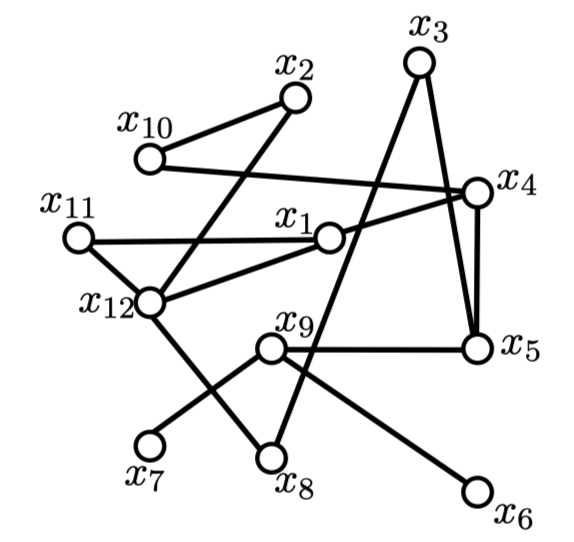
\includegraphics[width=0.4\textwidth]{Figs/1.png}
    \caption{Undirected pairwise graphical models example}
    \label{fig:Pairwise_Graph}
\end{figure}

\begin{itemize}
    \item Graph $G=(V, E)$
    \item Alphabet $\mathcal{X}$
    \item Compatibility function $\psi_{i j}: \mathcal{X} \times \mathcal{X} \rightarrow \mathbb{R}_{+}$, for all $(i, j) \in E$
\begin{align}
\mu(x)=\frac{1}{Z} \prod_{(i, j) \in E} \psi_{i j}\left(x_{i}, x_{j}\right)\label{eq:bdadc}
\end{align}
\item pairwise MRF only allow compatibility functions over two variables
\end{itemize}

\paragraph{Undirected General Graphical Models (MRF)}
The distrubtion function has been shown in \cref{eq:max_undir_graph}.

Consider a fixed graph $G(V, E)$
\begin{itemize}
    \item the factorizations implied by the graph under MRF and pairwise MRF are different, e.g. $\left(x_{1}, x_{11}, x_{12}\right)$
    \item independencies implied by the graph under MRF or pairwise MRF are the \tb{same}, however pairwise MRF represent \tb{less possible distributions}.
    \item by choosing the right compatibility functions any model represented by pairwise MRF can be represented by MRFs, \tb{but not the other way around}
\end{itemize}
\begin{rema}
Some MRF's do not factorize: a simple example can be constructed on a cycle of 4 nodes with some infinite energies, i.e. configurations of zero probabilities, even if one, more appropriately, allows the infinite energies to act on the complete graph on $V$.

MRF's factorize if at least one of the following conditions is fulfilled:
\begin{enumerate}
    \item the density is positive (by the Hammersley–Clifford theorem)
    \item the graph is chordal (by equivalence to a Bayesian network)
\end{enumerate}
\end{rema}

\paragraph{Conversion from General to Pairwise}\label{sec:con_gen_pair}
With \tb{additional nodes}, it is possible to describe how any Markov random field with discrete random variables can be converted to an equivalent pairwise form (i.e., with interactions only between pairs of variables). However, it still has flaw that cannot totally be written in the form of pure product as in \cref{eq:bdadc}. Summation is still needed to get the marginal.
\begin{proof}
To illustrate the general principle, it suffices to show how to convert a compatibility function $\psi_{123}$ defined on a triplet $\left\{x_{1}, x_{2}, x_{3}\right\}$ of random variables into a pairwise form. To do so, we introduce an auxiliary node $A$, and associate with it random variable $z$ that takes values in the Cartesian product space $\mathcal{X}_{1} \times \mathcal{X}_{2} \times \mathcal{X}_{3} .$ In this way, each configuration of $z$ can be identified with a triplet $\left(z_{1}, z_{2}, z_{3}\right)$. For each $s \in\{1,2,3\}$, we define a pairwise compatibility function $\psi_{A s}$, corresponding to the interaction between $z$ and $x_{s}$, by $\psi_{A s}\left(z, x_{s}\right):=\left[\psi_{123}\left(z_{1}, z_{2}, z_{3}\right)\right]^{1 / 3} \mathbb{I}\left[z_{s}=x_{s}\right] .$ (The purpose of the $1 / 3$ power is to incorporate $\psi_{123}$ with the correct exponent.) With this definition, it is straightforward to verify that the equivalence
\begin{align}
\psi_{123}\left(x_{1}, x_{2}, x_{3}\right)=\sum_{z} \prod_{s=1}^{3} \psi_{A s}\left(z, x_{s}\right)\label{eq:}
\end{align}
holds, so that our augmented model faithfully captures the interaction defined on the triplet $\left\{x_{1}, x_{2}, x_{3}\right\}$.
\end{proof}


\subsubsection{Factor Graph Models}
\begin{figure}[H]
    \centering
    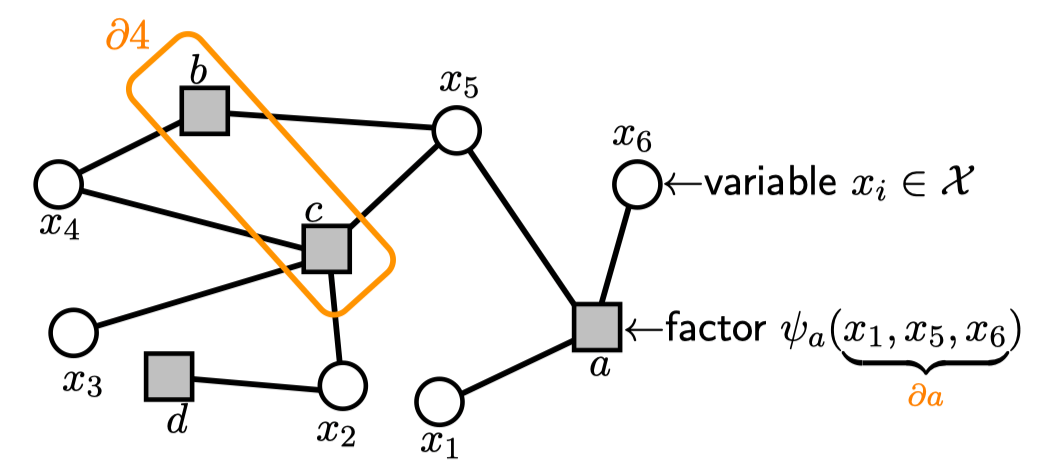
\includegraphics[width=0.6\textwidth]{Figs/2.png}
    \caption{Factor graph example.}
    \label{fig:factor_Graph}
\end{figure}
\begin{itemize}
    \item Factor graph $G=(V, F, E)$
    \item Variable nodes $i, j, k, \cdots \in V$, $x_{i} \in \mathcal{X}$, for all $i \in V$
    \item Function nodes $a, b, c, \cdots \in F$
    \item Function node $\psi_{a}: \mathcal{X}^{\partial a} \rightarrow \mathbb{R}_{+}$, for all $a \in F$
\begin{align}
    \mu(x)=\frac{1}{Z} \prod_{a \in F} \psi_{a}\left(x_{\partial a}\right)
\end{align}
\end{itemize}


\subsubsection{Conversion between Factor Graphs and Undirected  Graphical ModelsThe}
\boxx{
$\bullet$ \tb{From pairwise model to factor graph:}

A pairwise model on $G(V, E)$ with alphabet $\mathcal{X}$ can be represented by a
factor graph $G^{\prime}\left(V^{\prime}, F^{\prime}, E^{\prime}\right)$ with $V^{\prime}=V, F^{\prime} \simeq E,\left|E^{\prime}\right|=2|E|, \mathcal{X}^{\prime}=\mathcal{X}$.

$\diamond$ \tb{Key:} Put a factor node on each edge.}

\boxx{
$\bullet$ \tb{From factor graph to a general undirected graphical model (MRF):}

A factor model on $G(V, F, E)$ with alphabet $\mathcal{X}$ can be represented by a
MRF on $G^{\prime}\left(V^{\prime}, E^{\prime}\right)$ with $V^{\prime}=V, E^{\prime} \simeq \sum_{a \in F}|\partial a|^{2}, \mathcal{X}^{\prime}=\mathcal{X}$.

$\diamond$ \tb{Key:}  A factor node is turned into a clique.}

\boxx{
$\bullet$ \tb{From factor graph to a pairwise model:}

A factor model on $G(V, F, E)$ can be represented by a pairwise model on
$G^{\prime}\left(V^{\prime}, E^{\prime}\right)$ with $V^{\prime}=V \cup F, E^{\prime}=E, \mathcal{X}^{\prime}=\mathcal{X}^{\Delta}, \Delta=\max _{a \in F} \operatorname{deg}(a)$. Similar to \cref{sec:con_gen_pair}.

$\diamond$ \tb{Key:}A factor node is represented by a large variable node}

\begin{rema}\bfs{factor graphs vs. undirected graphical models}
Factor graphs are more ``fine grained'' than undirected graphical models
\begin{itemize}
    \item  \tb{set of independencies} represented by MRF is the same as FG
    \item but FG can represent a larger set of factorizations
\end{itemize}
\end{rema}

\begin{figure}[H]
    \centering
    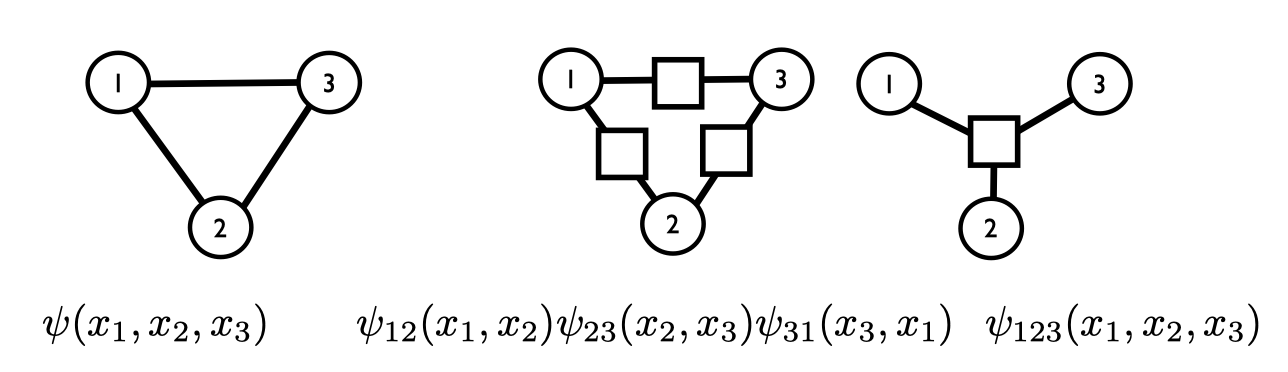
\includegraphics[width=0.8\textwidth]{Figs/3.png}
    \caption{MRF vs. Factor graph. All three encodes same independencies, but different factorizations (in particular the degrees of freedom in the compatibility functions are $3|\mathcal{X}|^{2}$ vs. $\left.|\mathcal{X}|^{3}\right)$}
    \label{fig:diff_fartor_ugm}
\end{figure}
\subsubsection{Bayesian Network (Directed Graphical Model)}

\begin{figure}[H]
    \centering
    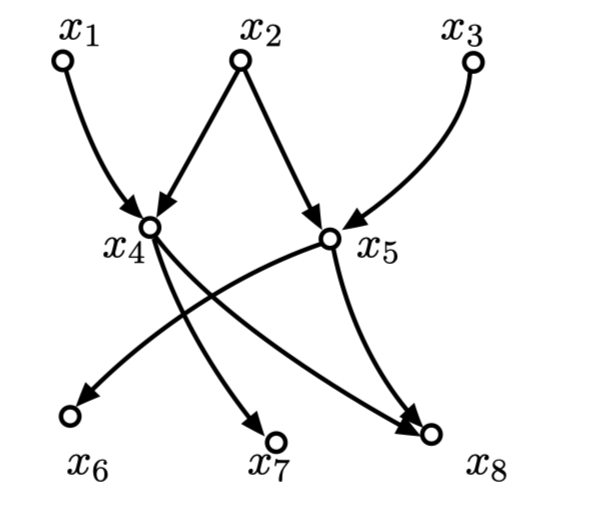
\includegraphics[width=0.5\textwidth]{Figs/4.png}
    \caption{Bayesian network example.}
    \label{fig:bayes1}
\end{figure}

Bayesian network is specified by
\begin{itemize}
    \item directed acyclic graph $G=(V, D)$
    \item alphabet $\mathcal{X}$
    \item conditional probability $\mu_{i}(\cdot \mid \cdot): \mathcal{X} \times \mathcal{X}^{\pi(i)} \rightarrow \mathbb{R}_{+}$, for $i \in V$
\begin{align*}
\mu(x)=\prod_{i \in V} \mu_{i}\left(x_{i} \mid x_{\pi(i)}\right)
\end{align*}
\item we do not need normalization $(1 / Z)$ since
\begin{align*}
\sum_{x_{i} \in \mathcal{X}} \mu_{i}\left(x_{i} \mid x_{\pi(i)}\right)=1 \Rightarrow \sum_{x \in \mathcal{X}^{V}} \mu(x)=1
\end{align*}
\end{itemize}

\begin{figure}[H]
    \centering
    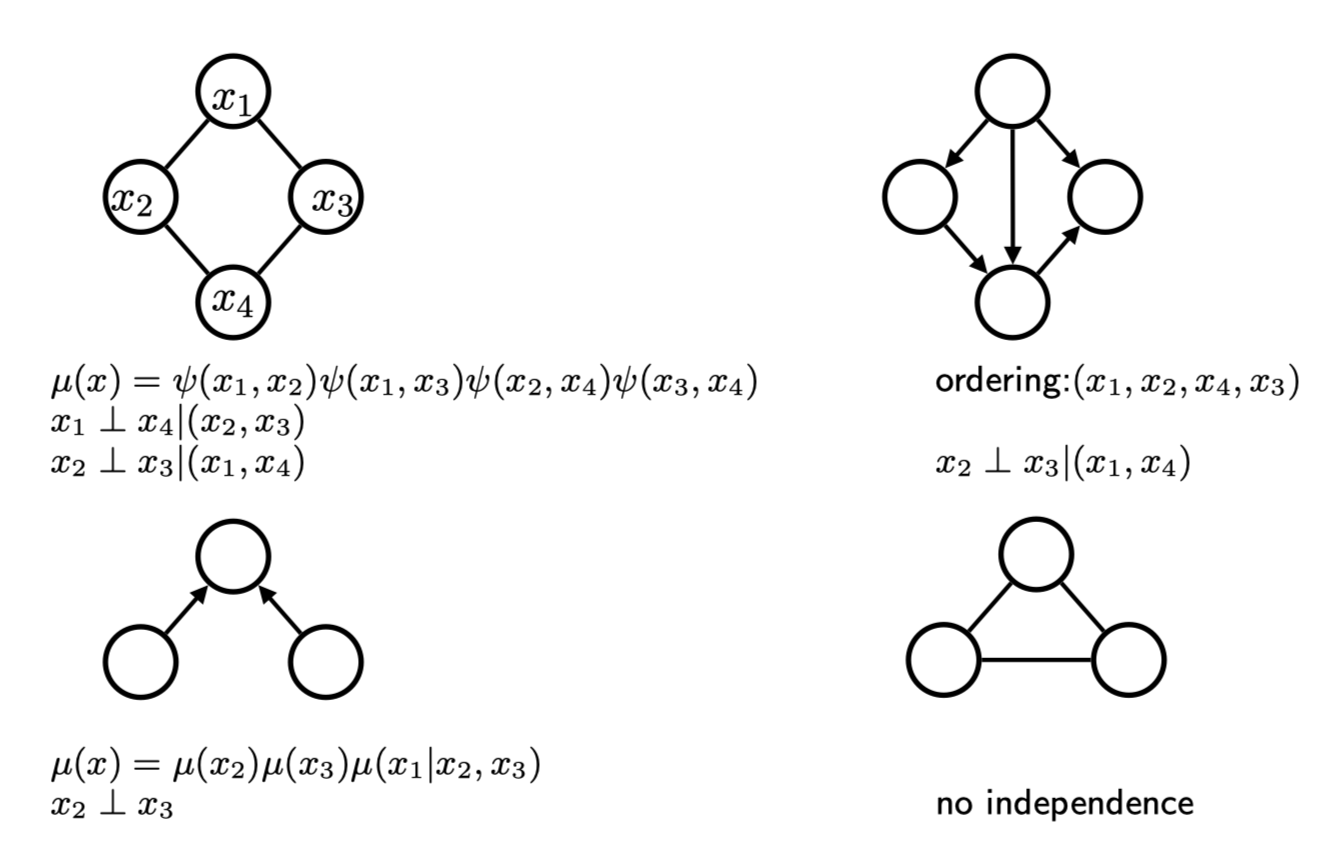
\includegraphics[width=0.7\textwidth]{Figs/5.png}
    \caption{MRF and BN are incomparable, some independence  is lost in conversion in both direction.}
    \label{fig:bayesvsmrf}
\end{figure}
\begin{exma}\bfs{Bayes networks with observed variables}
\begin{itemize}
    \item $V=H \cup O$
    \item  Hidden variables: $x=\left(x_{i}\right)_{i \in H}$
    \item Observed variables: $y=\left(y_{i}\right)_{i \in O}$
\begin{align*}
\mu(x, y)=\prod_{i \in H} \mu\left(x_{i} \mid x_{\pi(i) \cap H}, y_{\pi(i) \cap O}\right) \prod_{i \in O} \mu\left(y_{i} \mid x_{\pi(i) \cap H}, y_{\pi(i) \cap O}\right)
\end{align*}
\item Objective: 
Typically interested in $\mu_{y}(x) \equiv \mu(x \mid y)$ and
$\arg \max _{x} \mu_{y}(x)$
\end{itemize}
\end{exma}

\subsubsection{Conversion between Bayesian Networks and Factor Graphs}
In general because MRF and BN are incomparable, some independence structure will be lost in conversion.

\boxx{
$\bullet$ \tb{From Bayesian network to factor graph:}

A Bayes network $G=(V, D)$ with alphabet $\mathcal{X}$ can be represented by a factor graph model on $G^{\prime}=\left(V^{\prime}, F^{\prime}, E^{\prime}\right)$ with $V^{\prime}=V,\left|F^{\prime}\right|=|V|$, $\left|E^{\prime}\right|=|D|+|V|, \mathcal{X}^{\prime}=\mathcal{X} .$

$\diamond$ \tb{Key:}  

\begin{itemize}
    \item represent by a factor node each conditional probability
    moralization for conversion from BN to MRF (we will learn this)
\end{itemize}}

% \subsubsection{Graph Concepts from \cite{koller2009probabilistic}}


\boxx{
$\bullet$ \tb{
From factor graph to Bayesian network:}

A factor model on $G=(V, F, E)$ with alphabet $\mathcal{X}$ can be represented by a
Bayes network $G^{\prime}=\left(V^{\prime}, D^{\prime}\right)$ with $V^{\prime}=V$ and $\mathcal{X}^{\prime}=\mathcal{X}$.

$\diamond$ \tb{Key:} 

\begin{itemize}
    \item  take a topological ordering, e.g. $x_{1}, \ldots, x_{n}$
    \item for each node $i$, starting from the first node, find a minimal set $U \subseteq\{1, \ldots, i-1\}$ such that $x_{i}$ is conditionally independent of $x_{\{1, \ldots, i-1\} \backslash U}$ given $x_{U}$. (we will learn how to do this)
    \item in general the resulting Bayesian network is dense
\end{itemize}
}

\subsection{Markov Property}
\begin{exma}$$
\begin{gathered}
X-Y-Z \\
X \perp Z \mid Y \\
\mu(X, Y, Z)=f(X, Y) g(Y, Z)
\end{gathered}$$
\end{exma}
\begin{figure}[H]
    \centering
    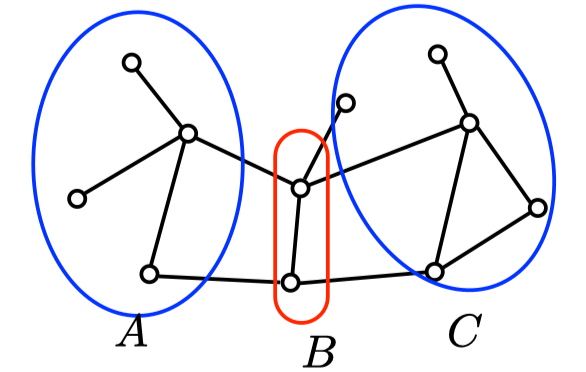
\includegraphics[width=0.6\textwidth]{Figs/6.png}
    \caption{Markov property.}
    \label{fig:Markov}
\end{figure}
Let $A \cup B \cup C$ be a partition of $V$, we have
\begin{defa}\bfs{Graph Separation}
 $B$ \tb{separates} $A$ from $C$ if any path starting in $A$ and terminating in $C$ has at least one node in $B$
\end{defa}
% \begin{defa}\bfs{Global Markov Property}
%  distribution $\mu$ over $\mathcal{X}^{V}$ satisfies the \tb{global Markov property} on $G$ if for \tb{any} partition $(A, B, C)$ such that $B$ separates $A$ from $C$,
% $$\mu\left(x_{A}, x_{C} \mid x_{B}\right)=\mu\left(x_{A} \mid x_{B}\right) \mu\left(x_{C} \mid x_{B}\right)$$
% \end{defa}

\subsubsection{Markov Property for Undirected Graphs}
\begin{defa}\bfs{Global Markov Property}
 We say $\mu(\cdot)$ satisfy the \tb{global Markov property ($\mathrm{G}$)} w.r.t. a graph $G$ if for any partition $(A, B, C)$ such that $B$ separates $A$ from $C$,
\begin{align*}
\mu\left(x_{A}, x_{C} \mid x_{B}\right)=\mu\left(x_{A} \mid x_{B}\right) \mu\left(x_{C} \mid x_{B}\right)
\end{align*}
\end{defa}
\begin{defa}\bfs{Local Markov Property}
 We say $\mu(\cdot)$ satisfy the \tb{local Markov property ($\mathrm{L}$)}  w.r.t. a graph $G$ if for any $i \in V$,
\begin{align*}
\mu\left(x_{i}, x_{\text {rest }} \mid x_{\partial i}\right)=\mu\left(x_{i} \mid x_{\partial i}\right) \mu\left(x_{\text {rest }} \mid x_{\partial i}\right)
\end{align*}
\end{defa}
\begin{defa}\bfs{Pairwise Markov Property}
 We say $\mu(\cdot)$ satisfy the \tb{pairwise Markov property  ($\mathrm{P}$)}  w.r.t. a graph $G$ if for any $i, j \in V$ that are \tb{not connected} by an edge
\begin{align*}
\mu\left(x_{i}, x_{j} \mid x_{\text {rest }}\right)=\mu\left(x_{i} \mid x_{\text {rest }}\right) \mu\left(x_{j} \mid x_{\text {rest }}\right)
\end{align*}
\end{defa}

\paragraph{Conditional Independence: Local, Global and Pairwise}
$\bullet$ \tb{In general:} $(\mathrm{G}) \Rightarrow(\mathrm{L}) \Rightarrow(\mathrm{P})$
We need the following lemma:
\begin{lema}\bfs{Conditional Independence Lemmas}\label{lem:gvdfsfz}
For any deterministic function $h(\cdot)$,
\begin{align}
X \perp Y \mid Z & \Longrightarrow \quad X \perp Y \mid(Z, h(Y)) \label{eq:hdfe}\\
X \perp Y \mid Z & \Longrightarrow \quad X \perp h(Y) \mid Z \label{eq:mbdre}
\end{align}
\end{lema}
\begin{rema}
See also \cite[Page 216]{durrett2019probability} for discussion of conditional independence, where it points out  
\centerline{``\tb{conditioning on a sub or sup sigma algebra, it is \tb{not} necessarily conditional independent}''.}

\end{rema}
\begin{cora}\label{cora:dfax}From \cref{lem:gvdfsfz}, we have
\begin{itemize} 
    \item Decomposition:
\begin{align*}
{X} \perp {Y}, {W} \mid {Z} \Longrightarrow {X} \perp {Y} \mid {Z}.
\end{align*}
\item Weak union:
\begin{align*}
{X} \perp {Y}, {W} \mid {Z} \Longrightarrow {X} \perp {Y} \mid {Z}, {W}
\end{align*}
\end{itemize}
In addition, we also have 
\begin{itemize}
\item Contraction:
\begin{align*}
{X} \perp {W} \mid {Z}, {Y} \text{ and } {X} \perp {Y} \mid {Z} \Longrightarrow {X} \perp {Y}, {W} \mid {Z}
\end{align*}
\end{itemize}
\end{cora}
\begin{proof} (of \cref{lem:gvdfsfz})
\begin{align*}
\begin{aligned}
\mu(x, y, h(Y)=h, z) &=\mu(x, y, z) \mathbb{I}(h(y)=h) \\
&=f(x, z) g(y, z) \mathbb{I}(h(y)=h)
\end{aligned}
\end{align*}
This implies both $X \perp(Y, h(Y)) \mid Z$ and $X \perp Y \mid(Z, h(Y))$.

$$\mu(x, h, z)=\sum_{y} \mu(x, y, h, z)=f(x, z) \underbrace{\sum_{y} g(y, z) \mathbb{I}(h(y)=h)}_{\tilde{g}(h, z)}.$$ This implies $X \perp h(Y) \mid Z$.
\end{proof}
\begin{proof} (of \cref{cora:dfax})
Decomposition is easy. Weak union is also easy: ${X} \perp {Y}, {W} \mid {Z} \Longrightarrow {X} \perp {Y}, W \mid {Z}, {W} \Longrightarrow {X} \perp {Y} \mid {Z}, {W}$.  For contraction, $\mu({X} \mid {Z}, {Y},W ) = \mu({X} \mid {Z}, Y ) = \mu({X} \mid {Z})$.
\end{proof}
\begin{proof} (of  $(\mathrm{G}) \Rightarrow(\mathrm{L}) \Rightarrow(\mathrm{P})$)

Obviously: $(\mathrm{G}) \Rightarrow(\mathrm{L})$. The proof of  $(\mathrm{L}) \Rightarrow(\mathrm{P})$ is directly from \cref{lem:gvdfsfz}: 

\cref{eq:hdfe} $\Longrightarrow$ $x_{i} \perp x_{\mathrm{rest}} \mid \left(x_{V \backslash\{i, j\}}\right) $, \cref{eq:mbdre} $\Longrightarrow$ $x_{i} \perp x_{\mathrm{rest}} \mid\left(x_{V \backslash\{i, j\}}\right)$
\end{proof}

$\bullet$ \tb{In general: $(\mathrm{P}) \nRightarrow (\mathrm{G})$}

But $(\mathrm{P}) \Rightarrow(\mathrm{G})$ if the following holds for all disjoint subsets $A, B, C$, and $D \subseteq V$ :
\begin{align}
   \text{``If $x_{A} \perp x_{B} \mid\left(x_{C}, x_{D}\right)$ and $x_{A} \perp x_{C} \mid\left(x_{B}, x_{D}\right)$, then $x_{A} \perp\left(x_{B}, x_{C}\right) \mid x_{D}$''}  \label{eq:hdfz}
\end{align}

\begin{lema}\bfs{Intersection Lemma}
For \tb{strictly positive probability distributions}, \tb{if $\mu(x)>0$ for all $x \in \mathcal{X}$}, the following  holds:
\begin{align*}
X \perp Y \mid Z, W   \text { and }  X \perp W \mid Z, Y \Rightarrow X \perp W, Y \mid Z
\end{align*}
\end{lema}
\begin{rema}
So if we add the strictly positive assumption, we can get \cref{eq:hdfz} and therefore $(\mathrm{P}) \Rightarrow(\mathrm{G})$. See below.
\end{rema}
\begin{proof}
By assumption:
\begin{align*}
\mu(X \mid Z, W, Y)=\mu(X \mid Z, W) \wedge \mu(X \mid Z, W, Y)=\mu(X \mid Z, Y) \Longrightarrow \mu(X \mid Z, Y)=\mu(X \mid Z, W)
\end{align*}
Using this equality, together with the law of total probability applied to $\mu(X \mid Z)$ :
\begin{align*}
\begin{aligned}
\mu(X \mid Z) &=\sum_{w \in W} \mu(X \mid Z, W=w) \mu(W=w \mid Z) \\
&=\sum_{w \in W} \mu(X \mid Y, Z) \mu(W=w \mid Z) \\
&=\mu(X \mid Z, Y) \sum_{w \in W} \mu(W=w \mid Z) \\
&=\mu(X \mid Z, Y)
\end{aligned}
\end{align*}
Since $\mu(X \mid Z, W, Y)=\mu(X \mid Z, Y)$ and $\mu(X \mid Z, Y)=\mu(X \mid Z)$, it follows that $\mu(X \mid Z, W, Y)=\mu(X \mid Z) \Longleftrightarrow X \perp Y, W \mid Z$.
\end{proof}

$\bullet$ \tb{Proof of $(\mathrm{P}) \Rightarrow(\mathrm{G})$ when \cref{eq:hdfz}  holds:}

\begin{figure}
    \centering
    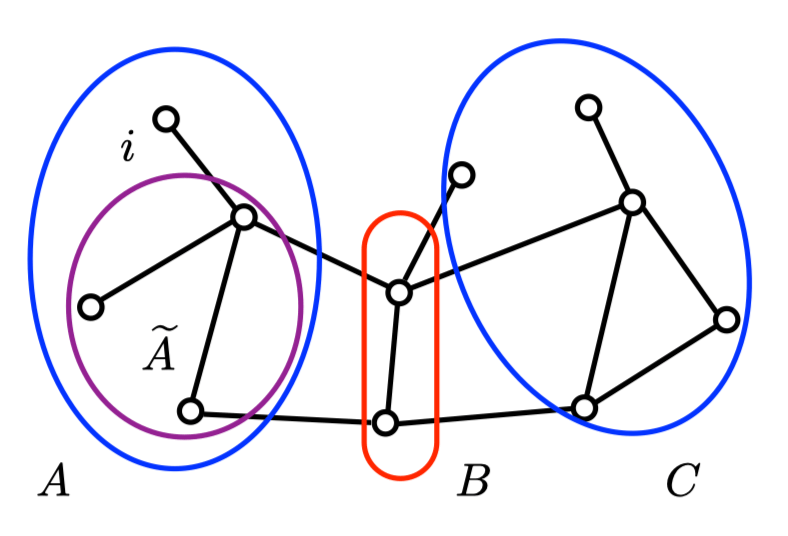
\includegraphics[width=0.5\textwidth]{Figs/7.png}
    \caption{ $(\mathrm{P}) \Rightarrow(\mathrm{G})$ }
    \label{fig:proofofptog}
\end{figure}
\begin{proof}
By induction over $s \triangleq|B|$:
\begin{enumerate}
    \item initial condition: when $s=n-2,(\mathrm{P}) \Leftrightarrow(\mathrm{G})$. (true from the definition)
    \item induction step:
assume $(\mathrm{G})$ for any $B$ with $|B| \geq s$ and prove it for $|B|=s-1$
\end{enumerate}
W.L.O.G, we consider a set $A$ with $|A| \geq 2$ and $B$ with $|B|=s$ (see \cref{fig:proofofptog}). By induction assumption, for any $i \in A$, we have
\begin{itemize}
    \item $x_{C} \perp x_{\widetilde{A}} \mid\left(x_{B}, x_{i}\right)$
    \item $x_{C} \perp x_{i} \mid\left(x_{B}, x_{\widetilde{A}}\right)$
\end{itemize}
 By  \cref{eq:hdfz}, we have 
    $x_{C} \perp\left(x_{\widetilde{A}}, x_{i}\right) \mid x_{B}$. By induction, we see that $(\mathrm{G})$ holds for all sizes of $B$.
\end{proof}

\paragraph{Hammersley-Clifford}
\begin{thma}\bfs{Hammersley-Clifford Theorem}\label{thm:ham_cliff}
A strictly positive distribution $\mu(x)$ (i.e. $\mu(x)>0$ for all $x$ ) satisfies the global Markov property $(\mathrm{G})$ with respect to $G(V, E)$ if and only if it can be factorized according to $G$ :
$$(\mathrm{F}): \quad \mu(x)=\frac{1}{Z} \prod_{c \in \mathcal{C}(\mathrm{G})} \psi_{c}\left(x_{c}\right)$$
\end{thma}
\begin{rema}
In other words, any $\mu(x)$ with Markov property can be represented with MRF. Note three Markov property  are equivalent to each other under the strictly positive distribution  assumption.
\end{rema}
\begin{proof}
$\diamond$  $(\mathrm{F}) \Rightarrow(\mathrm{G})$ easy

$\diamond$ $(\mathrm{F}) \Leftarrow(\mathrm{G})$ requires much more effort, and we first prove that  $(\mathrm{G})$ (i.e. $(\mathrm{P})$) implies the following:
\begin{itemize}
    \item For any  $A \subseteq V$ and pair $i, j$ of non-neighbouring nodes such that $i \notin A$ and $j \in A$,
\begin{align}
\frac{\mu(x_{A+i},0_{\mathrm{rest}})}{\mu(x_A,0_{\mathrm{rest}})+\mu(x_{A+i},0_{\mathrm{rest}})}=\frac{\mu(x_{A- j+i},0_{\mathrm{rest}})}{\mu(x_{A-j},0_{\mathrm{rest}})+\mu(x_{A-j+i},0_{\mathrm{rest}})}, \label{eq:dcdaweew}
\end{align}
where $\mu(A,0_{\mathrm{rest}})$ meaning the probability that all other nodes other than $A$ will have value $0$. Note here we assume the same alphabet $\calX$ for all nodes, if different $\calX_s$ for different $x\in V$, here we just change $0_{\mathrm{rest}}$ to one  vector than has one specific fixed value at one specific node.
\begin{align*}
\frac{\mu(x_{A+i},0_{\mathrm{rest}})}{\mu(x_A,0_{\mathrm{rest}})+\mu(x_{A+i},0_{\mathrm{rest}})} & = \frac{\mu(x_i \mid x_A, 0_{\mathrm{rest}})\mu(x_A, 0_{\mathrm{rest}}) }{\mu(x_A,0_{\mathrm{rest}})+\mu(x_i \mid x_A, 0_{\mathrm{rest}})\mu(x_A, 0_{\mathrm{rest}}) } \\
& = \frac{\mu(x_i \mid x_A, 0_{\mathrm{rest}}) }{1+\mu(x_i \mid x_A, 0_{\mathrm{rest}})}\\
& = \frac{\mu(x_i \mid x_{A-y}, 0_{\mathrm{rest}}) }{1+\mu(x_i \mid x_{A-y}, 0_{\mathrm{rest}})}\\
& = \frac{\mu(x_i \mid x_{A-y}, 0_{\mathrm{rest}})\mu(x_{A-y}, 0_{\mathrm{rest}}) }{\mu(x_{A-y}, 0_{\mathrm{rest}})+\mu(x_i \mid x_{A-y}, 0_{\mathrm{rest}})\mu(x_{A-y}, 0_{\mathrm{rest}})}\\
& = \frac{\mu(x_{A- j+i},0_{\mathrm{rest}})}{\mu(x_{A-j},0_{\mathrm{rest}})+\mu(x_{A-j+i},0_{\mathrm{rest}})}\\
\end{align*}
\end{itemize}
where the strictly positive has been used in the division and the third equality is from $\mathrm{P}$.

(Above we prove $(\mathrm{G})\Rightarrow$ \cref{eq:dcdaweew}, we actually have $(\mathrm{G})\Leftrightarrow$ \cref{eq:dcdaweew} after we notice the third equality $\frac{1}{1+x}$ is a 1-1 mapping.)

For simplicity of notation in the proof, in the following we always use the letter $c$ to represent a typical clique.

Suppose first that $V: \calX^B \rightarrow \mathbb{R}$ is defined by
\begin{align}
    V(x_{A},0_{\mathrm{rest}})\coloneqq \sum_{B \subseteq A}(-1)^{|A-B|} \log \mu(x_{B},0_{\mathrm{rest}}),\text{ for all } A \subseteq V\label{eq:mweqrz3rg}
\end{align}
% Let $\omega \in \Omega$ and $A \subseteq L(\omega) .$ Then, by (6),
% \begin{align*}
% V(\omega A)=\sum_{B \subseteq A}(-1)^{|A-B|} \log \mu(\omega B)
% \end{align*}y
\tb{We first claim that $V(x_{A},0_{\mathrm{rest}})=0$ unless $A$ is a clique}. For, suppose $A$ contains two sites $i, j$ which are not neighbours. Then, from \cref{eq:dcdaweew}, we have
\begin{align*}
V(x_{A},0_{\mathrm{rest}})=& \sum_{B \subseteq A \atop i, j \in B}(-1)^{|A-B|} \log \mu(x_{B},0_{\mathrm{rest}}) + \sum_{B \subseteq A \atop i \in B, j \notin B}(-1)^{|A-B|} \log \mu(x_{B},0_{\mathrm{rest}})\\
&+\sum_{B \subseteq A \atop i\notin B, j \in B}(-1)^{|A-B|} \log \mu(x_{B},0_{\mathrm{rest}})+\sum_{B \subseteq A \atop i, j \notin B}(-1)^{|A-B|} \log \mu(x_{B},0_{\mathrm{rest}}) \\
=& \sum_{B \subseteq A-i-j}(-1)^{|A-B|} \log \left(\frac{\mu(x_{B+j+i},0_{\mathrm{rest}})}{\mu(x_{B+j},0_{\mathrm{rest}}))} / \frac{\mu(x_{B+i},0_{\mathrm{rest}})}{\mu(x_{B},0_{\mathrm{rest}})}\right) \\
=& 0.
\end{align*}
The set of subsets is partially ordered by inclusion, and its \tb{M\"obius function} $\mu$ is given by
\begin{align*}
\mu(B, A)=(-1)^{|A-B|}
\end{align*}
We write \cref{eq:mweqrz3rg} in the form
\begin{align*}
 V(x_{A},0_{\mathrm{rest}})=\sum_{B \subseteq A} \mu(B, A) \log \mu(x_{B},0_{\mathrm{rest}})
\end{align*}
which yields
\begin{align*}
\log \mu(x_{A},0_{\mathrm{rest}})=\sum_{B \subseteq A}  V(x_{B},0_{\mathrm{rest}})
\end{align*}
by the {M\"obius Inversion Theorem} in \cref{thm:mobius}. Hence, by the above claim about clique,
\begin{align*}
\mu(x)= \exp \left(\sum_{c\in \calC(G)} V(x_c, 0_{\mathrm{rest}})\right) 
\end{align*}
Let $\psi_{c}\left(x_{c}\right) \coloneqq  \exp \big(V(x_c, 0_{\mathrm{rest}})\big)$. The proof is now complete.
\end{proof}
\begin{rema}\bfs{definition consistence}
In \cref{eq:mweqrz3rg}, it seems there exists some ambiguous, since we may add more nodes taking $0$ to $A$ to get a larger set and the sum in the left side is over a larger set. However, please note here the additional sum is $0$, so it does not matter whether we should let $x_A$ contain $0$. And it is a consistent definition.
\end{rema}
% \begin{align*}
% \mu(x)= \exp \left(\sum_{c\in \calC(G) \text{ and $x_c$ takes no $0$}} V(x_c, 0_{\mathrm{rest}})\right) 
% \end{align*}
% \begin{rema}
% Some explanation of ``Let $\psi_{c}\left(x_{c}\right) \coloneqq  \exp \big(\frac{1}{t_c}V(x_c, 0_{\mathrm{rest}})\big)$.'' 
% \begin{itemize}
%     \item In some sense, we are \tb{iterating over all cliques that takes no $0$ value.} 
%     \item  When $c$ iterates over all cliques $\calC(G)$,  if $x_c$ has $0$ inside, we need to rule out the nodes that takes value $0$ and look at $V(x'_c, 0_{\mathrm{rest}})$.
%     \begin{enumerate}
%         \item If now the left nodes are not connected as a clique, we know $V(x'_c, 0_{\mathrm{rest}})=0$. 
%         \item If now the left nodes are connected as a sub-clique, note that the sub-clique will be counted twice or more during the iteration over all cliques $\calC(G)$. In this case, we need to count how many time, denoted as times $t_c$, $x'_c$ will be counted in the iteration and do a average when define $\psi_{c}$.
%     \end{enumerate}
% \end{itemize}
% \end{rema}
Here I introduce one interesting theorem named M\"obius inversion formula which will be used in the proof of \cref{thm:ham_cliff} above.
\begin{thma}\bfs{M\"obius Inversion Theorem}\label{thm:mobius}
For a poset $P$, a set endowed with a partial order relation $\leq$, define the \tb{M\"obius function} $\mu$ of $P$ recursively by 
$$\mu(s, s)=1 \text{  for  } s \in P, \quad \mu(s, u)=-\sum_{s \leq t< u} \mu(s, t), \text{ for }s<u \text{ in }P .$$
(Here one assumes the summations are finite.) Then for $f, g: P \rightarrow K$, where $K$ is a commutative ring, we have
$$g(t)=\sum_{s \leq t} f(s) \quad\text{ for all } t \in P$$
if and only if
\begin{align*}
f(t)=\sum_{s \leq t} g(s) \mu(s, t) \quad \text { for all } t \in P .
\end{align*}
\end{thma}
\begin{rema}\bfs{explanation}
A partially ordered set (poset) $P$ is a set with a relation $\leq$ that is
\begin{itemize}
    \item Reflexive: $x \leq x$ holds for all $x \in P$;
    \item Antisymmetric: if $x \leq y$ and $y \leq x$ then $x=y$;
    \item Transitive: if $x \leq y$ and $y \leq z$ then $x \leq z$.
\end{itemize}
Examples of partially ordered sets include: the subsets of a set, ordered by inclusion, the real numbers, ordered by the usual $\leq$ relation, and the natural numbers, ordered by the relation "divides".

An equivalent condition for \tb{M\"obius function} $\mu$ of $P$:
$$\mu(s, s)=1 \text{  for  } s \in P, \quad \sum_{s \leq t\le u} \mu(s, t)=0, \text{ for }s<u \text{ in }P .$$

If $P$ is the set of all finites subsets of the set $\{1,2,3, \ldots\}$, ordered by inclusion, then the M\"obius function is $\mu(X, Y)=(-1)^{|Y|-|X|}$. (W.L.O.G., we assume $s=\{1\}$ and $u=\{1,2,...,n\}$. Then $\sum_{s \leq t\le u} \mu(s, t)=(1-1)^{n-1}=0$ (from combination $(1+a)^n$, set $a=-1$) , for $s<u$.)

The M\"obius inversion formula implies
\begin{align*}
g(X)=\sum_{Y \subseteq X} f(Y) \quad \text { iff } \quad f(X)=\sum_{Y \subseteq X} g(Y)(-1)^{|X|-|Y|}
\end{align*}
and, for all subsets of $\{1,2, \ldots, n\}$,
\begin{align*}
g(X)=\sum_{\{1, \ldots, n\} \supset Y \supset X} f(Y) \text { iff } f(X)=\sum_{\{1, \ldots, n\} \supset Y \supset X} g(Y)(-1)^{|Y|-|X|} .
\end{align*}
\end{rema}
\begin{proof}
We show that $g(t)=\sum_{s \leq t} f(s)$ if and only if $f(t)=\sum_{s \leq t} g(s) \mu(s, t)$, the proof of the other statement is similar. The statement makes sense only if we assume that for any $x$ only finitely many $y$ 's satisfy $y \leq x$. Let us fix an element $x_{0}$ and consider only elements that are less than or equal to $x_{0}$. We may assume this is our entire poset $P$. 

Let us associate to $P$ a square matrix $Z$ whose rows and columns are indexed with the elements of $P$, and which \tb{has a $1$ in row $x$, column $y$ exactly when $x \leq y$, and has a zero in all other rows:} 

\emph{Multiplying the row vector $\underline{f}:=(f(y) \mid y \in P)$ with the matrix $Z$ from the right yields a row vector whose entry associated to $x$ is $\sum_{y \leq x} f(y)$.}

Let us introduce $\underline{g}:=(g(x) \mid x \in P)$, and the matrix $M$ whose \tb{entry in row $x$ and column $y$ is $\mu(x, y)$ if $x \leq y$ and zero otherwise}. The  statement in \cref{thm:mobius} is equivalent to saying
\begin{align*}
\underline{g}=\underline{f} \ast Z \quad \text { if and only if } \quad \underline{f}=\underline{g} \ast M .
\end{align*}
This is obviously true if the matrices $M$ and $Z$ are inverses of each other, so it suffices to show
\begin{align*}
I=M \ast Z
\end{align*}
To verify this we need to check that the product of a row indexed by $x$ in $M$ and a row indexed by $y$ in $Z$ is $\delta_{x, y}$, the Kronecker delta function. In other words we need to check
\begin{align*}
\sum_{x \leq z \leq y} \mu(x, z)=\delta_{x, y}
\end{align*}
which is exactly the definition of the Möbius function.
\end{proof}
\subsubsection{Markov Property of Directed Graphical Models}
See ``Graphical Models Notes''



\bibliographystyle{IEEEtran}
\bibliography{IEEEabrv,StringDefinitions,adv_dnn}
\end{document}